\documentclass[11pt]{article}
\usepackage[margin=1.1in]{geometry}
\usepackage{amsmath,amssymb}
\usepackage[protrusion=true,expansion=false]{microtype}
\usepackage{xcolor}
\usepackage{enumitem}
\usepackage{tikz}
\usepackage{float}
\usetikzlibrary{arrows.meta}
\usepackage{hyperref}

\hypersetup{pdftitle={Licash: ecash with a unilateral exit to Bitcoin}, colorlinks=true, linkcolor=blue!60!black, urlcolor=blue!60!black, citecolor=blue!60!black}
\usepackage[skip=0.6\baselineskip, indent=0pt]{parskip}

\makeatletter
\renewcommand\section{\@startsection{section}{1}{\z@}{-2.5ex plus -1ex minus -.2ex}{1.2ex plus .2ex}{\large\bfseries}}
\renewcommand\@seccntformat[1]{\csname the#1\endcsname.\hspace{0.7em}}
\makeatother

\newcommand{\paperversion}{0.14}

\newcommand{\vmax}{V_{\max}}
\newcommand{\wH}{w_H}
\newcommand{\wP}{w_P}
\newcommand{\wA}{w_A}
\newcommand{\wC}{w_C}
\newcommand{\wX}{w_X}
\newcommand{\tx}[1]{\texttt{#1}}
\newcommand{\Ht}[1]{H_{\mathsf{#1}}}
\newcommand{\htc}{\mathsf{h2c}}
\newcommand{\id}{\mathsf{id}}
\newcommand{\bresp}{b'}
\newcommand{\DLEQ}{\mathsf{DLEQ}}
\newcommand{\G}{\mathcal{G}}
\newcommand{\prop}[2]{\paragraph{Property #1 (#2).}}

\definecolor{coop}{RGB}{232,245,233}
\definecolor{hubc}{RGB}{255,243,214}

\title{\textbf{Licash}\\ecash with a unilateral exit to Bitcoin}
\author{m0wer \and waxwing}
\date{Version \paperversion, November 2026}

\begin{document}
\maketitle

\begin{abstract}
Licash is ecash in which every holder has an individual right to redeem their notes for bitcoin from the issuer, the \emph{hub}, on Bitcoin itself, without the hub's cooperation. Payments are offchain reissuances between one-time keys: they are immediate, use no blockspace and leave no public trace, and the hub cannot link the spending of a note to its issuance. A holder recovers by publishing a claim to her own notes. The burden of proof is on the hub: the claim is paid in full unless the hub shows, with a spend the holder authorized, that she is owed less, and proves it on Bitcoin if she contests. A wallet therefore never produces a proof, never reads shared state and need not be online to be paid within its hub, and a claim from a stale backup is paid exactly its unspent part. Payments are atomic without trust, because the hub can use a payer's signature against her only by publishing the key that releases the payee's notes. The same rule, publish the secret or pay the refund, connects a hub to onchain Bitcoin, to Lightning and to other hubs.
\end{abstract}

\section{Introduction}

Bitcoin payments are public and compete for blockspace. Receiving to fresh addresses helps little once the coins are spent together, because consolidation links its inputs, and the change of each payment links it to the next. Our goal is to move routine payments and the merging of value offchain, so that they are private, cheap and fast, while every user keeps the ability to recover their money on Bitcoin without anyone's cooperation, even from a phone.

Ecash~\cite{chaum,cashu,fedimint} is private and cheap, but custodial: users trust the mint with their money. Designs with unilateral exit usually judge an exit against shared state, such as a transaction tree~\cite{ark} or nullifiers reconstructed from Bitcoin~\cite{shieldedcsv,shieldedbitcoin}, which must be ordered and available to everyone. Lichen~\cite{lichen} instead gives each user a bilateral Bitcoin contract with an operator. In a dispute, the contract's transactions verify a Groth16 proof with BABE~\cite{babe}, one of several ways, after BitVM~\cite{bitvm,bitvm2} and other garbled-circuit designs~\cite{bitvm3,glock}, to verify a proof on Bitcoin without changing its rules.

Licash\footnote{From ``lichen ecash,'' pronounced ``lee cash.''} uses such contracts to back ecash whose value on Bitcoin rests on a signature by each note's key alone. A payment reissues value to one-time keys that only the recipient controls, without naming any account or contract. To recover, the holder lists her own notes in a Bitcoin transaction and signs for each with its key. She does not prove that the notes are unspent. The hub, which keeps the record of spends, must prove that a listed note was spent, and the only proof it can give is a spend that the holder signed. Recovery is therefore \emph{local}: it concerns only the holder's notes and her contract.

This puts the burden of proof on the party that has the data, the resources and the reason to refute a claim, and an honest claim is paid without anyone proving anything. A wallet's part is mostly signing, and it can be paid by another user of its hub while offline.

Paying offchain is a fair exchange, impossible without a trusted third party~\cite{fairexchange}. As in~\cite{andrychowicz,bentov}, that party is Bitcoin, used only in a dispute. The hub must release a secret to \emph{prevent} the payer from recovering her inputs, and that secret pays the payee and returns the payer's change. A note spend locked under a hash carries the same rule, publish the secret or pay the refund, to onchain Bitcoin, to Lightning and to other hubs.

\paragraph{Related designs.} These designs also differ in what they ask of a user. A self-custodial Lightning user~\cite{lightning} maintains channels with inbound capacity, is online to receive, and monitors the chain for revoked states, herself or through a watchtower. Ark users receive without managing liquidity, but must renew their outputs of the shared tree before they expire, or exit by broadcasting their path of it. An Ark user paid outside a round must also refresh the payment in a round before it is safe from a sender colluding with the operator. In Shielded CSV, a recipient verifies a proof of each coin she receives and scans Bitcoin for published nullifiers. A Licash user does none of these, and has the recovery right of a channel without its watching. The cap of her contracts limits how much she can recover, not, as a channel's capacity does, what she can receive: she holds any balance above the cap on trust, as at a mint.

The difference is also one of privacy. Routing nodes see the hops they forward, and channel balances and the endpoints of payments can be inferred~\cite{kappos}. An Ark operator learns the inputs, outputs and amounts of the transfers it cosigns~\cite{arkformal}. A Licash hub sees which notes are spent together, but cannot link a note's spending to its issuance. Cashu's pay-to-public-key conditions~\cite{nut11} also bind ecash to a recipient's key, but only the mint enforces them. In Licash that key is what the holder claims with on Bitcoin.

\paragraph{Contributions.}
\begin{itemize}[leftmargin=1.5em, itemsep=0pt]
\item \emph{Recovery that the hub must disprove.} A claim lists the holder's notes, designated by one-time keys and not bound to an identity, and is paid unless the hub proves that some were spent, which leaves the holder's part light enough for a phone (Sections~\ref{sec:rec} and~\ref{sec:light}).
\item \emph{Grants.} The payee's notes are encrypted under a key that the hub must publish to use the payer's signature against her, which makes an offchain payment atomic (Section~\ref{sec:pay}).
\item \emph{Timed locks.} Hash-locked payments with forced publication of the preimage give swaps, Lightning payments and payments between hubs (Section~\ref{sec:interop}).
\item \emph{Unlinking.} A perfectly blinded proof of correct issuance unlinks a note's spending from its issuance (Section~\ref{sec:model}).
\end{itemize}

\section{Model}
\label{sec:model}

\paragraph{Parties.} The hub issues notes and co-funds its users' contracts. It may refuse service, withhold answers, issue notes it should not, collude with users or disappear. Users may double spend, claim notes they have spent and collude with each other. The cryptographic assumptions are listed in Section~\ref{sec:security}. Each party keeps its own records.

\paragraph{Bitcoin.} A proof sees Bitcoin only as block headers, and cannot tell them from headers mined in private. We therefore assume that, from a user's request until the hub's deadline to assert, no party can mine in private a chain with the work that her contract requires. One such chain could serve every dispute open at that time, so a hub sets the required work in proportion to the total value that its contracts protect. We also assume that no block buried as deep as a contract or a lock requires is reorganized, and that a party that must act on Bitcoin by a deadline can get a transaction confirmed within a known number of blocks, paying for it from the contract's fee reserve or from its own coins.

\paragraph{Notation.} $G$ is the secp256k1 generator; lowercase scalars multiply uppercase points. A denomination $d$, a power of two in satoshis, selects the hub's secret key $k_d$ with public key $K_d=k_dG$. $\DLEQ(G,K;B,C)$ is a Chaum-Pedersen proof~\cite{chaumpedersen} that $K=kG$ and $C=kB$ for the same $k$. $H_{\mathsf{tag}}$ are tagged hashes, and $\htc$ hashes to the curve~\cite{rfc9380}. The hub also has a signing key, for the certificates of Section~\ref{sec:interop}.

\paragraph{Notes.} As in Cashu~\cite{cashu}, a note is a message $x$ with a point $C=k_dY$, where $Y=\htc(x)$ is the note's \emph{identifier}. To issue it, the holder sends $B=Y+rG$ for a random $r$, the hub returns $C'=k_dB$ with $\DLEQ(G,K_d;B,C')$, and the holder computes $C=C'-rK_d$. A note is \emph{settled} once its holder has a proof that $C=k_dY$, the note's \emph{issuance proof}. The hub keeps a private \emph{spend log}: the identifiers it has seen spent, each with the spend that consumed it.

\paragraph{Owner keys.} A user has independent spend, scan and hold keys $b_s,b_v,b_h$, and $(B_s,B_v,B_h)$ is their address. A payer picks an ephemeral key $A=aG$ and derives output $j$ as in silent payments~\cite{bip352}:
\begin{gather*}
\varsigma = \Ht{ecdh}(\mathsf{xcoord}(aB_v)),\qquad s_j = \Ht{seed}(\varsigma, j),\\
P_j = B_s + \Ht{tweak}(B_s, s_j)\,G,\qquad Q_j = B_h + \Ht{hold}(B_h,B_s,s_j)\,G,\\
x_j = (d_j, P_j, Q_j),\qquad B_j = \htc(x_j) + r_jG,
\end{gather*}
with the blinding $r_j$ also derived from $\varsigma$. Unlike in Cashu, the message has no nonce, since $P_j$ is used once. The payer draws $A$ anew for each spend, since the same $A$ to the same recipient would give the same outputs, which the hub issues once. The recipient recomputes both keys from $A$ before accepting an output. Only she can sign for the \emph{owner key} $P_j$, which authorizes spending the note, and for the \emph{hold key} $Q_j$, which authorizes claiming it on Bitcoin. Change is derived the same way and is not marked as change. Neither key reveals the address or any other note of its owner.

\paragraph{Unlinking.} The proof received at issuance contains $B$, so it would link a later spend to that issuance. At any time after issuance, the holder can replace it with a proof on $(Y,C)$, made in a separate session with the hub in which the Chaum-Pedersen protocol is blinded the way one blinds a Schnorr signature. With the issuance the hub sends $(R_1,R_2)=(wG,wB)$ for a nonce $w$. To unlink, the holder picks blinding scalars $\alpha,\beta$ and sends the blinded challenge $\gamma$:
\[
R_1' = R_1 + \alpha G + \beta K_d,\quad R_2' = R_2 - rR_1 + \alpha Y + \beta C,\quad \gamma' = \Ht{dleq}(R_1', R_2', K_d, Y, C),\quad \gamma = \gamma' + \beta .
\]
The hub answers $s=w+\gamma k_d$, and never answers a second challenge under the same nonce: two answers would reveal $k_d$. Then $(\gamma',s+\alpha)$ is a valid proof of $\DLEQ(G,K_d;Y,C)$. The hub learns which of its issuances were unlinked, but since $\alpha$ and $\beta$ are uniform, every completed session is equally likely to have produced any given unlinked proof: the blinding is perfect. Either proof serves as the note's issuance proof. If the hub refuses to unlink, the note keeps its value and the proof that links it to its issuance.

\paragraph{Contracts.} A contract is a Bitcoin output that a user and the hub fund together and can spend only together, as in Lichen~\cite{lichen}. Before it is funded they sign the transactions that may spend it, the contract's \emph{graph}: one with which the user starts a recovery, those of the dispute that may follow (Section~\ref{sec:rec}), and one that returns the funds to the hub when the contract expires. The dispute rests on BABE~\cite{babe}: the user prepares garbled circuits that verify a Groth16 proof of the hub, so that in a dispute the hub must prove its case or lose it. The amounts paid are not fixed in advance: each party signs the amount it asks for with a one-time signature~\cite{delving}.

The output holds the funds that back the contract, whose size is its cap $\vmax$, the most that a recovery can pay, and a fee reserve from each party. The user funds her reserve, her part of the cap and the hub's price. The hub funds the rest of the cap, and the price is in proportion to what it funds and for how long. Her part is owed to her as notes, and the hub's part is what lets her recover notes that she receives later.

What is specific to Licash is in the contract's \emph{terms}: the hub's note keys, the cap, both parties' keys, the program of the hub's statement (Section~\ref{sec:rec}), the \emph{checkpoint} block from which that program reads Bitcoin and the work it requires, how many items a claim may list, and the windows of the dispute in blocks: publication $\wP$, response $\wH$, contest $\wX$, assertion $\wA$ and challenge $\wC$. A digest $D$ binds the terms to the graph, and both parties check it before the funding transaction is signed.

\paragraph{Opening is atomic.} The user pays for her part of the cap in the funding transaction, and the hub owes her notes of that value. A hub that took her funding and never issued them would leave her with nothing to claim. So, before the funding transaction is signed, she sends the hub blinded outputs worth her part, derived as for a payment to herself, and the contract's terms include a hash of their list. These are her \emph{funded notes}. The hub has not yet issued them, but the contract's rules count them as valid notes: once the funding is confirmed, she can claim them in a recovery (Section~\ref{sec:rec}) without an issuance proof, by showing the list and how each claimed note opens its entry. The hub therefore has no reason to withhold them, and issues them as ordinary notes once the funding has a few confirmations.

\paragraph{What a contract covers.} A contract lets its holder redeem notes worth $b$ satoshis, up to the cap, for $b$ satoshis paid from the contract output: in a recovery (Section~\ref{sec:rec}) if the hub does not cooperate, or in a close that both sign (below). Apart from her funded notes, the terms do not tie the contract to particular notes. She only has to sign with the hold keys of the notes that she redeems, so notes that she received before the contract existed are redeemed like any others, and notes are issued and spent without reference to a contract. Receiving a payment within a hub therefore does not require a contract, and it does not require the recipient to be online: the payer needs only her address, and she finds the payment later (Section~\ref{sec:pay}). The restriction is that a contract pays once: it supports one recovery, of one amount $b$, and a note can be claimed in only one of the contracts that its holder has with the note's hub. A holder's notes are \emph{protected} while their value fits in her open contracts. Value beyond that is held on trust, as at a mint, until she spends it or a further contract covers it, and a balance smaller than the fees of a recovery cannot in practice be recovered.

\paragraph{Expiry and closing.} Each contract has an expiry, after which a transaction of its graph returns the contract's funds to the hub, except the holder's reserve. It pays the reserve to an output that the terms fix, an HTLC~\cite{htlc}: the hub can take it with a preimage that only the holder knows, and the holder can take it back after a delay. This lets her receive the reserve as notes. She asks the hub to lock notes to her under the same hash (Section~\ref{sec:interop}), worth the reserve less a fee that the terms fix, and by revealing the preimage she takes those notes and lets the hub take the coins. This way the expiry does not pay a coin to her onchain wallet, which would link the contract to her other coins. If she never asks, or the hub is gone, she takes the coins back after the delay.

The holder must act while a recovery can still finish. The \emph{last safe action} is the latest height at which a request still leaves every window of the dispute before the expiry. Before it, she spends her notes, protects them with a newer contract or recovers.

The two parties can also close a contract together earlier, and the holder is then paid her claim in the same transaction, up to the cap. She gives the hub the claim she would file, and either the hub cosigns, or it shows her the evidence that it would use against some notes (Section~\ref{sec:rec}). She checks it as the statement would, so each side knows how an onchain dispute would end, and both can agree on the corrected claim without running it. A note that the hub calls spent without showing evidence stays in her claim, which she then files on Bitcoin.

\section{Payments}
\label{sec:pay}

A \emph{spend} $S$ lists input notes, blinded outputs $(B_j,d_j)$ of the same total value and the payer's ephemeral key $A$. Its identifier $\id(S)$ is a hash of all of it. A spend is authorized by a signature under the owner key of every input. When the hub accepts an authorized spend it records the inputs as spent and issues the outputs. A hub that charges a fee is paid by an output of the spend, addressed to it like any other, so the values of a spend always balance.

If the hub issued the outputs only after recording the spend, it could record Alice's signed payment and withhold Bob's notes. Alice's inputs would be spent, on evidence that she signed herself, and Bob would be unpaid. A \emph{grant} removes the gap. The hub issues every output before the payer signs, sealed under a key that it can use against the payer only by publishing it (Figure~\ref{fig:grant}).
\begin{enumerate}[leftmargin=1.8em, itemsep=0pt]
\item Alice sends the unsigned spend $S$ to the hub.
\item The hub draws a secret scalar, the \emph{unlock} $t$, with \emph{unlock key} $T=tG$. For every output $j$ it hashes $\id(S)$ and $j$ to a curve point $U_j$, and computes the \emph{sealed note} $\tilde C_j$ with a proof $\sigma_j$:
\[
\tilde C_j = k_{d_j}B_j + tU_j,\qquad \sigma_j = \mathsf{PoK}\{(k_{d_j},t) : K_{d_j}=k_{d_j}G,\ T=tG,\ \tilde C_j=k_{d_j}B_j+tU_j\}.
\]
The proof is a Schnorr proof of knowledge of both secrets, and its challenge also hashes the output's unlinking commitment $(R_1,R_2)$ (Section~\ref{sec:model}). The hub returns the grant $\G = \big(\id(S),\ T,\ (d_j,B_j,\tilde C_j,\sigma_j)_j\big)$, which also carries those commitments.
\item Alice verifies every $\sigma_j$ and that $\G$ lists her outputs, then signs $\Ht{auth}(\id(S), \mathsf{com}(T, \G))$ with each input's owner key, where $\mathsf{com}$ hashes $T$ and the whole grant. Her authorization is valid for this grant only.
\item The hub records the authorized spend and releases $t$.
\item Alice sends $S$, $\G$ and $t$ to Bob. He checks $tG=T$ and every $\sigma_j$, and with the blinding $r_j$, which he derives as she did (Section~\ref{sec:model}), he computes $C_j=\tilde C_j-tU_j-r_jK_{d_j}$, which $\sigma_j$ shows to be $k_{d_j}Y_j$.
\end{enumerate}

\begin{figure}[H]
\centering
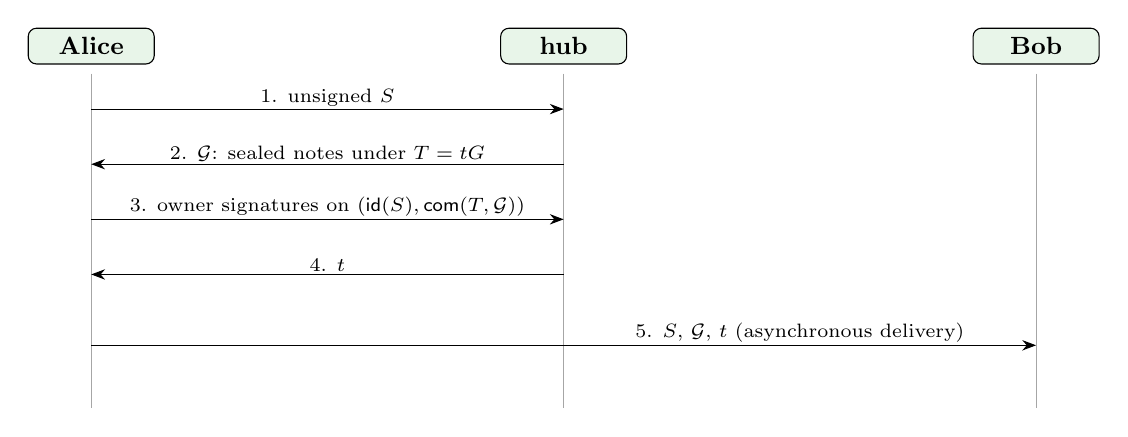
\begin{tikzpicture}[font=\small, >={Stealth[length=5pt]}, msg/.style={font=\scriptsize, fill=white, inner sep=1pt}]
\foreach \x/\n in {0/Alice, 6/hub, 12/Bob} {
  \node[draw, rounded corners=3pt, fill=coop, minimum width=16mm] at (\x,0) {\textbf{\n}};
  \draw[black!35] (\x,-0.35) -- (\x,-4.6);
}
\draw[->] (0,-0.8) -- node[msg, above] {1. unsigned $S$} (6,-0.8);
\draw[->] (6,-1.5) -- node[msg, above] {2. $\G$: sealed notes under $T=tG$} (0,-1.5);
\draw[->] (0,-2.2) -- node[msg, above] {3. owner signatures on $(\id(S), \mathsf{com}(T,\G))$} (6,-2.2);
\draw[->] (6,-2.9) -- node[msg, above] {4. $t$} (0,-2.9);
\draw[->] (0,-3.8) -- node[msg, above, pos=0.75] {5. $S$, $\G$, $t$ (asynchronous delivery)} (12,-3.8);
\end{tikzpicture}
\caption{A granted payment.}
\label{fig:grant}
\end{figure}

An opened note has $\sigma_j$ as its issuance proof: given $t$, $r_j$ and $U_j$, anyone recomputes $B_j$, $\tilde C_j$ and $T$ from $(Y_j,C_j)$ and verifies $\sigma_j$ under the ordinary key $K_{d_j}$. Its holder unlinks it like any other note. Bob treats a payment as settled when he holds $t$ and his outputs open. Before that the grant is of no use to him: to remove the term $tU_j$ without $t$, he would have to compute it from $T$ and $U_j$, which is the Diffie-Hellman problem.

Alice verifies the sealed notes before she signs: each $\sigma_j$ shows that the discrete logarithm of $T$ opens $\tilde C_j$ to her output, without her knowing $t$. The hub can use her signature against her only by citing her spend in a recovery, and it can cite a granted spend only by publishing a $t$ with $tG=T$ (Section~\ref{sec:rec}), which opens every sealed note. Whoever checks such a citation therefore checks one equation for the grant, $tG=T$, however many outputs the spend has.

Bob need not be online when Alice pays: she keeps the payment until he acknowledges it, and a mailbox or the hub can relay it. Once paid, Bob unlinks the notes. Alice, who derived them, still recognizes them until he respends them to outputs that only he can derive (Section~\ref{sec:privacy}).

A spend whose outputs all return to the spender, such as a consolidation or a change of denominations, is granted like any other. Until the hub releases its unlock, the spender can claim its outputs as fallbacks (Section~\ref{sec:rec}).

\section{Recovery}
\label{sec:rec}

\paragraph{The claim.} A holder starts a recovery with two transactions. The \emph{request} belongs to the contract's graph, so both parties signed it before the funding. It spends the contract output and carries her one-time signatures on two values, an amount $b$ and a 32-byte \emph{claim digest} $E$. One of its outputs is the \emph{slot}: the holder can spend it at any time with a key that the terms fix, and the hub can spend it $\wP$ blocks after the request confirms, when the publication window has passed. The \emph{publication} is the holder's spend of the slot, which she signs alone when she claims. It has an \texttt{OP\_RETURN} output that holds the claim that $E$ commits to and the data that supports it (below). Her signature covers that output, so nobody else can replace the claim, and so does the transaction's identifier, so the hub's program reads the claim from a block by a Merkle path. Data in a witness would be covered by neither. If she leaves the slot unspent, the hub spends it after the window. Either way one transaction spends the slot and the program reads which one, so whether a claim was published is settled on Bitcoin, and a request whose slot the hub took is owed nothing.

A claim lists items of four kinds, at most a number that the contract's terms fix (Section~\ref{sec:model}):
\begin{itemize}[leftmargin=1.5em, itemsep=0pt]
\item a \emph{settled note};
\item a \emph{fallback}: an output of a spend that the holder signed and has not seen completed, all of whose inputs are claimed as settled notes. A fallback is not counted in $b$. It stands in for those inputs if the hub turns out to have recorded the spend;
\item an output of a \emph{timed lock} (Section~\ref{sec:interop});
\item a \emph{funded note}: one of the outputs that the terms commit to for the part of the cap that she funded, whether or not the hub issued it.
\end{itemize}
The digest $E$ is a hash of the contract's digest $D$, the hub's note keys, $b$, the items, the spends, locks and activations that the items refer to, and the public fields of every note whose hold key must sign. It leaves out the signatures themselves. Each item carries a \emph{hold authorization}, a BIP340 signature under its hold key $Q_j$ over the note's public fields, $D$, $b$ and $E$. That signature is the whole of the authority to recover the item: the claim does not name an address and does not contain a proof. The publication holds, after the claim, the data that lets anyone check it: the issuance proof of each settled note, the body of each spend or lock whose outputs it claims, and the Bitcoin inclusion of any lock activation that it relies on. The amount satisfies $b \le \min(\vmax, \sum_{i\notin F} d_i)$, where $F$ is the set of fallbacks.

\paragraph{The size of a claim.} Notes have fixed denominations, so a wallet that receives many payments holds many notes, and the publication that lists them is a Bitcoin transaction. The limit on items keeps it small enough to be relayed and the proof of a dispute affordable. In the current implementation a claim lists up to 32 items and takes at most about 13~kvB, well below the standard transaction limit. A recovery that is not disputed is about 15~kvB in all; the hub's assertion of a proof adds about 8~kvB, and a challenge, made only against a false proof, about 20~kvB. The hub's proof takes about ten minutes on a consumer GPU. Notes beyond the limit, as after receiving offline, are held on trust until the wallet merges them with the hub. Merging may cost the hub's fee and shows the hub that the notes belong together, so a wallet merges notes after they rest, and sooner as it nears the limit.

Once a publication confirms, the hub records the notes and outputs that it claims as spent, before it decides on the claim. Whatever the holder is paid, she has given up her claimed notes for it, so no note is paid both on Bitcoin and by the hub. The hub keeps each claim's hold authorizations, to cite against a claim of the same notes in another contract. A contract pays once, so within one contract a later claim replaces an earlier one.

\paragraph{What a claim is owed.} A malformed claim is the holder's error and is owed nothing. An invalid \emph{item}, such as a note that the hub did not issue or a hold signature that is not by its note's hold key, is worth nothing, and the rest of the claim is still owed. A claim without such faults is owed $b$, unless the hub holds \emph{evidence} against it, of three kinds. Against notes and fallbacks the evidence is a signature of the claimant, and against the outputs of a lock it is the resolution of that lock:
\begin{itemize}[leftmargin=1.5em, itemsep=0pt]
\item $\mathsf{Spend}(S)$: an owner-authorized spend $S$. It voids the claimed notes that it consumes, and the claimed outputs of any other spend or lock that shares an input with it. The hub cites it by giving the bytes of $S$, which hash to $\id(S)$, and the owner signatures of only the inputs that matter to the claim: each input of $S$ that the claim lists, every input of $S$ if the claim lists outputs of $S$, and one input that $S$ shares with each other spend or lock whose outputs it voids. Only these signatures are verified. The rest of $S$ is hashed and not otherwise read, so citing a large spend costs little more than citing a small one;
\item $\mathsf{Claim}(E')$: a hold authorization of a claimed note for a claim in another contract, published or not. It voids that note, and what its payer claims of a lock that the note funds;
\item $\mathsf{Preimage}(z)$, which voids the refund outputs of a timed lock (Section~\ref{sec:interop}).
\end{itemize}
Each piece of evidence must void an item or cite the spend of a fallback. With $M$ the set of voided items, the fallbacks of every cited spend take the place of its voided inputs, and the claim is owed
\[
\bresp = \min\Big(b,\ \sum_{i \notin M,\ i \notin F} d_i \;+ \sum_{i \in F \setminus M,\ \text{spend of } i \text{ cited}} d_i\Big).
\]
There is no penalty. A claim made from an old backup is not fraud, and it is paid exactly the value that is still unspent: a claim of 3072 of which 1024 was spent is paid 2048. The change of a spend made after the backup can be claimed only as a fallback of that spend, so a wallet stores every spend before signing it.

\paragraph{Mandatory disclosure.} The hub must not retire a payer's inputs while keeping the payee's notes sealed. Citing a granted spend therefore requires its unlock $t$, with $tG=T$, which opens every sealed note of the grant: its payer verified them before signing. Since the owners signed $\mathsf{com}(T,\G)$, a granted spend cannot be cited without its grant's key. The hub must publish on Bitcoin every unlock and preimage that its evidence uses, and a wallet contests a response whose secrets are not all published.

\paragraph{The dispute.} The contract's graph is BABE with the roles of Lichen~\cite[App.~A]{lichen}: the hub proves and the holder verifies (Figure~\ref{fig:dispute}). When the hub has no evidence against a claim, it lets its response window $\wH$ pass and the claim is paid $b$. Otherwise it \emph{responds}, with a transaction of the graph that carries its one-time signature on an amount $\bresp<b$. This \emph{response} has a slot too, which only the hub can spend, and the hub's \emph{disclosure} spends it to publish, in an \texttt{OP\_RETURN} output, the secrets that its evidence uses. A response of $b$ would only keep the hub's reserve from an honest claim. The hub then shows the holder the evidence it responded on, and her wallet decides what the claim is owed from that evidence, her own filing and the chain, as the hub's statement would. If the claim is owed at most $\bresp$ and the secrets were disclosed, she lets her contest window $\wX$ pass and is paid $\bresp$ without anyone proving anything. Otherwise she \emph{contests}, and the hub must \emph{assert}, within $\wA$ blocks, a proof of its statement:
\begin{quote}
\emph{the claim published under this contract is owed at most $\bresp$, and the disclosure holds every secret that the evidence uses.}
\end{quote}
The hub \emph{flags} each item of the claim that it finds invalid, and the statement verifies those items and no others, taking the rest as valid, which can only raise what the claim is owed. The holder's wallet checks the asserted proof, and challenges a false one within $\wC$ blocks. BABE lets the hub answer a challenge only with a valid proof.

A proof decides a predicate, yet the dispute pays an amount. The hub therefore chooses $\bresp$ when it responds, from zero for a worthless claim to just below $b$, and proves that the claim is owed at most $\bresp$. A recovery thus ends in one of two payouts, $b$ or $\bresp$, though it can pay any value.

The terms fix the statement's program. It reads the request, the spend of its slot, the response and the disclosure from blocks whose headers extend the contract's checkpoint, with the required work on top of the last of them (Appendix~\ref{app:graph}). It checks the request's one-time signatures against keys that the terms fix, so a proof can be made only once the holder has requested. It takes $\bresp$ and the secrets as it finds them in those blocks, since a signature of the hub would prove nothing to a program that the hub runs. The proof is therefore about the amount that is paid, and about secrets that anyone can read, only if those blocks are Bitcoin's. Blocks with another publication, response or disclosure would have to be mined in private during the dispute, with the required work on top, which the model excludes. The program judges the claim on that chain up to the publication's block.

Here Licash departs from Lichen's simpler designs, whose proofs take their inputs only from one-time signatures, which cost blockspace for every bit signed. The holder signs only $b$ and $E$ that way, and the program reads the claim, kilobytes long, from Bitcoin and verifies its Schnorr hold signatures and issuance proofs itself. Checking a header costs the proof little next to the curve operations of a single note.

The hub proves its header chain ahead of any dispute, recursively, from a block a little below the first checkpoint it uses: the proof of each batch of headers verifies the proof of the batch before it and commits to every block's hash, its validity and the work up to it. Each contract's checkpoint is a block of that chain. The statement verifies the latest such proof, opens the few blocks it reads, the checkpoint among them, and checks the headers after it. Its cost therefore does not depend on the contract's age, and one chain proof serves every contract of the hub.

\begin{figure}[htb]
\centering
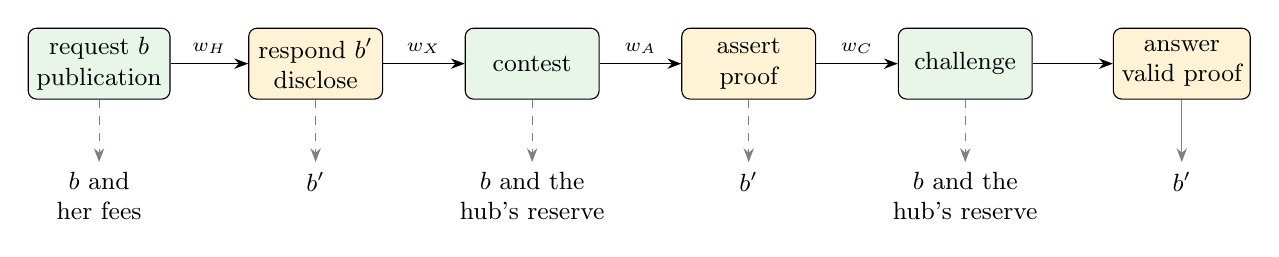
\begin{tikzpicture}[font=\small, >={Stealth[length=5pt]},
  box/.style={draw, rounded corners=3pt, inner sep=3pt, align=center, minimum width=17mm, minimum height=9mm},
  hold/.style={box, fill=coop}, hub/.style={box, fill=hubc},
  pay/.style={align=center, text=black}, win/.style={font=\scriptsize, above}]
\foreach \n/\s/\t [count=\i from 0] in {req/hold/{request $b$\\publication}, resp/hub/{respond $\bresp$\\disclose}, con/hold/{contest}, as/hub/{assert\\proof}, ch/hold/{challenge}, ans/hub/{answer\\valid proof}} {
  \node[\s] (\n) at (2.75*\i,0) {\t};
}
\foreach \a/\b/\w in {req/resp/$\wH$, resp/con/$\wX$, con/as/$\wA$, as/ch/$\wC$, ch/ans/{}} {
  \draw[->] (\a) -- node[win] {\w} (\b);
}
\foreach \n/\p in {req/{$b$ and\\her fees}, resp/{$\bresp$}, con/{$b$ and the\\hub's reserve}, as/{$\bresp$}, ch/{$b$ and the\\hub's reserve}} {
  \draw[->, black!50, dashed] (\n) -- ++(0,-1.25) node[pay, below] {\p};
}
\draw[->, black!50] (ans) -- ++(0,-1.25) node[pay, below] {$\bresp$};
\end{tikzpicture}
\caption{A recovery. Green moves are the holder's, yellow ones the hub's, each within the window above the arrow that leads to it. A dashed arrow is the timeout taken when the next move does not come, with what it pays the holder.}
\label{fig:dispute}
\end{figure}

The pattern is simple: if the hub does not move, the holder is paid $b$, and if the holder does not, she is paid $\bresp$. A hub that does not respond keeps the rest of its reserve, since it may have been kept from answering, by a flood of requests say, and a holder gains nothing from silencing it beyond her claim; a hub that responds and then fails to assert or to answer forfeits its reserve too. Each timeout is a transaction that pays only once it confirms, so a move that confirms first, even late, stands. A payout is signed before the funding, when its amount is not known. As in Lichen~\cite[Section~5.2]{lichen}, it has one output for each binary digit of the amount, and the one-time signature on $b$ or $\bresp$ decides which party can spend each. Digits below about 500 sats would make dust outputs and have none, so a payout is rounded down to that unit. The holder takes her outputs of a payout of $\bresp$ within a delay, after which the hub could take them by signing a second amount. Each party pays the fees of its own moves and can raise them after signing, so a rise in fees does not delay a move.

\paragraph{Incentives.} A reduced claim is not penalized, so that a stale backup is never punished, and neither is a contest. A holder who overstates a claim therefore risks only the fees of her own transactions, and she can impose on the hub the cost of responding and proving. A hub that responds but cannot prove forfeits its reserve, so it responds only with an amount that it can prove in time. Holders who file false claims in many contracts at once gain only if the hub cannot prove them all within the windows. Checking a claim against the spend log is cheap, so in a mass exit the hub responds only to the claims it knows to be overstated and proves them in order of their deadlines. It opens no more contracts than it can defend at once.

\paragraph{Example.} Alice holds notes of 2048 and 1024. She pays Bob 512 from the first, with change of 1024 and 512, under a grant. The hub records her signed spend and withholds $t$. Alice claims both notes for 3072 and lists the two change outputs as fallbacks. If the hub does nothing she is paid 3072 and the payment never happened. To do better the hub must cite her spend, which publishes $t$: the 2048 note is voided, the change takes its place, Alice is paid $1024+1536=2560$, and Bob opens his 512 with the published $t$. The hub cannot tell an honest Alice whose answer was withheld from a dishonest Alice claiming a note she spent, and it does not need to: both are paid what they are owed.

\section{Interoperability}
\label{sec:interop}

Value enters a hub when a contract opens and leaves it in a recovery or a close (Sections~\ref{sec:model} and~\ref{sec:rec}). Every other exchange with the outside, with onchain Bitcoin, Lightning or another hub, uses one mechanism. A \emph{timed lock} is a spend with two sets of outputs and terms $(h, e, \delta)$: the \emph{pay} outputs are issued to the payee if a preimage $z$ of $h$ is shown before Bitcoin height $e$, and the \emph{refund} outputs are issued to the payer otherwise. It does not need a grant, because neither set is issued until the lock settles. Anything else that pays under the same hash, a Bitcoin HTLC~\cite{htlc}, a Lightning invoice or a lock at another hub, can then be exchanged for notes atomically. The hub signs a \emph{certificate} of each lock it accepts, its acknowledgment of the debt to the payee. An honest hub issues the pay outputs when it learns $z$ before $e$, and the refund outputs once it has seen the chain reach height $e+\delta$ with the lock unactivated. Against a hub that does neither, three rules apply on Bitcoin.
\begin{itemize}[leftmargin=1.5em, itemsep=0pt]
\item \emph{Refund.} The payer claims the refund outputs, with a hold authorization for each input of the lock, in a claim judged on a chain that reaches height $e+\delta$; filed earlier, they are owed nothing and given up like any claimed output. Apart from what she signed herself, only $\mathsf{Preimage}(z)$ voids them, and the hub must then publish $z$. The payer is refunded or reads $z$ from Bitcoin.
\item \emph{Activation.} The payee can publish $z$ in a Bitcoin transaction. If it confirms below height $e$ and reaches depth $\delta$, the lock is \emph{activated}. The payee's claim of the pay outputs carries the activation, and cannot be voided by another spend of the lock's inputs.
\item \emph{Expiry.} Pay outputs claimed without an activation are owed nothing. A claim is judged on the chain up to its publication, which may confirm before the lock's fate is settled, while an activation settles it on Bitcoin.
\end{itemize}
A payee therefore keeps the lock's body, certificate and payer's signatures, and reveals $z$ to the hub only with at least $g$ blocks and a margin left before $e$, counted at a height she knows from a source other than the hub, while she can still activate. If the hub then keeps her notes, she activates and claims the pay outputs in her next recovery at that hub. By height $e+\delta$ any activation has reached depth $\delta$, so the hub holds $z$ when it answers a refund claim, however short the contract's response window. Only a lock whose pay outputs are all the hub's own may be refunded earlier offchain, when the hub gives up its claim to them. Either party relies on a lock only through contracts whose last safe action comes after $e+\delta$.

The lock's terms also name the hub's checkpoint of the period, a block deep in the chain that it shares among its locks and contracts of that period and on whose chain the lock's heights are read, and the pay outputs can be claimed in any contract of the payee's opened on that checkpoint or an earlier one.

\paragraph{Onchain swaps.} To sell notes for bitcoin, Alice picks $z$ and locks notes to a provider under $h$. The provider funds a Bitcoin HTLC that pays Alice with $z$ and refunds him before $e$. Alice takes the HTLC, which reveals $z$ on Bitcoin, and the provider collects the pay outputs, activating the lock if the hub does not answer. To buy notes with bitcoin, Alice funds an HTLC that pays the provider with $z$, and the provider locks notes to her with an earlier expiry. Alice reveals $z$ to the hub for her notes, or activates the lock, which publishes $z$ for the provider. The provider may be the hub itself, locking a note that it issued to itself, which lets a new user buy her first notes without a contract.

\paragraph{Lightning.} A hub that runs a Lightning node~\cite{lightning}, or a provider with a node and notes at the hub, is a \emph{gateway}. To pay an invoice, Alice locks notes to a gateway under its hash, and the gateway pays the invoice along routes that expire before $e$. The preimage is Alice's proof of payment, and if the hub keeps it, her refund request forces it onto Bitcoin. To be paid, Alice draws $z$ and has her hub issue a hold invoice under $h$, and when the payment arrives the hub locks a note of its own to her, expiring before the incoming HTLC. Alice reveals $z$ to the hub, or activates the lock, and the hub settles the invoice with it. Where an activation would cost more than the payment, she trusts the hub with it, as with value beyond her contracts. A recipient who is offline cannot reveal $z$ in time, so she is paid from Lightning only online, or through a provider that she trusts to receive for her and pay her later in notes.

\paragraph{Between hubs.} Value moves between hubs mainly over Lightning. To pay Bob at another hub, Alice pays a hold invoice of Bob's hub, under Bob's hash, through a gateway at her own hub, and Bob's hub locks its notes to him. Neither hub holds notes of the other, no party needs notes at both, and the two hubs do not need an arrangement between them.

Hubs can also be connected directly by ecash, without Lightning. A \emph{forwarder}, a provider or a hub, holds notes and a contract at a hub that it does not run, and a payment is one lock per hub under a common hash: at the recipient's hub it pays the recipient, and at each other hub the forwarder toward her. Routes of many hops do not need a further mechanism, but they need route discovery, fees for each hop and a way to hide the route from forwarders, which we leave open. A forwarder trades a Lightning channel for notes held at another hub, which only its contracts there protect.

Every exchange in this section rests on one ordering rule. A party has an incoming leg, which pays it, and an outgoing leg, which it pays, under one hash, and it holds $z$ within $\Delta$ blocks of the outgoing leg's expiry. If it issues the outgoing lock itself, or the outgoing leg is a Lightning or Bitcoin HTLC, its payee can settle only by revealing $z$ to it or on Bitcoin, and $\Delta=q$, the time to read $z$ from Bitcoin. If another hub issues the outgoing lock, that hub can keep $z$ from it, and the party overcomes that only with a refund request, owed from $e+\delta$. Then $\Delta$ adds the lock's depth $\delta$, the hub's response window and the request's confirmation. The incoming leg is safe if it outlives the outgoing one by the time to act on $z$, with $g$ blocks to confirm an activation and a margin $m$:
\[
e_{\mathrm{in}} > e_{\mathrm{out}} + \Delta + g + m.
\]
Whichever leg settles first expires first, so the party between them is paid whenever it pays.

\section{Light clients}
\label{sec:light}

Because the hub carries the burden of proof, a Licash wallet does very little, and almost all of it is ordinary signing.
\begin{itemize}[leftmargin=1.5em, itemsep=0pt]
\item \emph{To pay and be paid}, it derives one-time keys, signs spends and verifies the hub's issuance proofs.
\item \emph{Between payments}, it keeps its notes and a seed. It does not track a ledger or watch the Bitcoin chain, because nothing that another party publishes can reduce its claim. It only has to come back online before the last safe action of each contract.
\item \emph{To open a contract}, it garbles the BABE instances for the hub's statement once and uploads those the hub keeps. It keeps only the seed they derive from.
\item \emph{To recover}, it publishes a claim with the notes and spends it already holds, checks the hub's response and any asserted proof, and collects its payout. It must be online at each deadline of the dispute, and pays its fees from the contract's reserve.
\end{itemize}
Because a note is claimed with its hold key alone, any of her contracts with its hub can recover it, including one opened after she received it, and because a claim is reduced only by her own signatures, she need not know which of her notes are still unspent to claim them safely. The one duty that cannot be delegated without trust is the challenge, because the secrets that a challenge reveals would let a colluding hub answer any challenge~\cite[App.~A]{lichen}. It arises only in a dispute that the holder started, against a hub that asserts a false proof.

\section{Security}
\label{sec:security}

We assume that the discrete logarithm problem is hard in secp256k1, and so is the one-more gap Diffie-Hellman problem~\cite{jkk,privacypass}, against an adversary with two further kinds of access to the hub. It may run the interactive Chaum-Pedersen protocol with the hub on points whose evaluation the hub has released to it. It may also obtain any number of evaluations sealed as in a grant (Section~\ref{sec:pay}) and choose afterwards which of them the hub opens, and only the opened ones count as evaluations. This second extension is specific to grants, and we do not reduce it to the plain problem (Property~1). Tagged hashes are random oracles, BIP340 signatures are unforgeable~\cite{bip340}, the hub's statement is proven by a knowledge-sound zkVM with a Groth16 wrapper~\cite{risc0,groth16} whose setup had at least one honest contributor, and BABE is sound~\cite{babe}. Bitcoin behaves as Section~\ref{sec:model} assumes. A contract's statement is fixed at opening, so a flaw found in any of these is answered by closing contracts and opening new ones under a corrected statement. The arguments below are sketches in the random oracle model, not full proofs. A holder or hub is \emph{honest} if it follows the protocol, keeps its records and acts on Bitcoin within its deadlines.

\prop{1}{Issuance} An issuance proof that verifies, in any of its three forms, shows $C=k_dY$, and a coalition to whom the hub has released $\ell$ notes of denomination $d$ holds valid issuance proofs for at most $\ell$ identifiers of that denomination.

\emph{Argument.} The proof received at issuance and the unlinked proof are Fiat-Shamir transcripts of the Chaum-Pedersen protocol, and the proof of an opened note (Section~\ref{sec:pay}) is a Schnorr proof of the same kind for two secrets. All three are sound without computational assumptions, and their challenge hashes the whole statement, including $B$ or $Y$, so a false statement verifies with negligible probability. For an opened note the verifier recomputes $B=Y+rG$, $T=tG$ and $\tilde C=C+rK_d+tU$. Since $K_d$ and $T$ fix $k_d$ and $t$, the proof shows that $\tilde C=k_dB+tU$, which is $C=k_dY$ whatever point $U$ is. Proofs for $\ell+1$ identifiers would then solve the one-more gap Diffie-Hellman problem, whose decision oracle would in practice be the hub itself, reached over the network, if the rest of the coalition's view is simulatable without $k_d$. It is: issuance proofs are zero knowledge, and an unlinking session is the interactive prover of our assumption, a Schnorr identification of $K_d$~\cite{bellarepalacio} blinded as in blind Schnorr signatures~\cite{fps}. Concurrent-session attacks~\cite{ros} forge a signature on a new message, while a transcript here verifies only for a pair $(Y,k_dY)$, and a second proof of a note is not another note. A grant is a sealed evaluation of our assumption, with proofs that are zero knowledge, so it counts only if its unlock is released. We do not reduce this case to the plain problem: a sealed note binds the hub to $k_dB_j$ before the coalition decides whether to complete the spend, so a reduction would have to guess that decision for every grant. Our reason to believe the assumption is that, in the generic group model, the term $tU_j$ of a sealed note occurs only in that note, so without $t$ the note does not help to compute $k_dB_j$. The hub releases a note only against inputs of the same value or a payment it received, so valid unspent notes never exceed the value it was paid to issue.

\prop{2}{Holder recovery} An honest holder who claims protected notes worth $b$ before the last safe action of her contract is paid $b$, up to rounding and the fees of her own transactions, unless the hub shows her, and proves if she contests, that she is owed a smaller amount $\bresp$. She is then paid $\bresp$, every piece of the hub's evidence is an authorization that she signed or the resolution of a lock that she entered, and every unlock or preimage that the evidence uses is published on Bitcoin.

\emph{Argument.} Her items are valid, so none is flagged, and her claim is owed $b$ unless evidence voids an item. The statement reads her own request and publication, and the hub's response and disclosure, on Bitcoin's chain by the assumption on private work. If the hub does not respond, is contested and does not assert, or cannot answer her challenge, the graph pays $b$. An honest wallet lets a response pass only when the hub's evidence bears it out, which it verifies itself. If she contests and the hub asserts a valid proof, the statement shows that the claim is owed at most $\bresp$ under evidence that verifies and was disclosed. A $\mathsf{Spend}$ carries signatures under her owner keys, and a $\mathsf{Claim}$ a signature under her hold key, neither of which can be forged. An honest holder claims each note in one contract only, so only spends she signed reduce her claim, and for each of them her fallbacks count her change. Her funded notes, issued or not, are voided likewise only by her own signatures. Lock outputs are covered by Property~5.

\prop{3}{Hub safety} An honest hub that opens no more contracts than it can defend at once pays each note at most once, by reissuing it or on Bitcoin, and pays at most $\vmax$ per contract.

\emph{Argument.} Every item of a claim is valid, or the hub proves it invalid and it is worth nothing, so a claim is paid only for notes that the hub issued (Property~1) or owes for the part of the cap its holder funded, which the terms commit to, and for each one in its spend log the hub holds the owner-signed spend. The hub issues the funded notes only once the funding transaction is confirmed, so it never owes them for a contract that did not open. A claim does not name an owner, so a note may be claimed in two contracts, but each claim's hold authorization voids the note in the other: a holder who claims twice is paid nothing for it. A contract's funds leave it once on Bitcoin, so of the claims of one contract only the one its exit carries is ever paid. Once a claim is published the hub records its notes as spent, and cites it against any claim of them in another contract. The hub can prove in time every claim that it can reduce, so none is paid by a timeout. A fallback counts only when its spend is cited, in place of inputs of the same value. The two sides of a lock are never both paid (Property~5), and $b$ is signed below the cap. The statement is a deterministic function of Bitcoin and the hub's evidence, so an honest hub evaluates it before responding and never responds with an amount it cannot prove.

\prop{4}{Payment atomicity} If Alice, with protected inputs, signs a granted spend that pays Bob, then either the hub never counts her inputs as spent and she recovers them in full, or the unlock $t$ reaches her or Bitcoin, every sealed note opens (she verified each before signing), Bob can open his outputs and Alice holds her change.

\emph{Argument.} Alice's signature covers $\mathsf{com}(T,\G)$, so it authorizes this grant and no other spend of her inputs, and she signs only once every $\sigma_j$ verifies, so that by the soundness of the proofs the discrete logarithm of $T$ opens each $\tilde C_j$. If the hub releases $t$, the payment completes. Otherwise Alice claims her inputs with her change as fallbacks. By Property~2 she is paid in full unless the hub cites her spend, which requires publishing the $t$ with $tG=T$, so one that opens every sealed note. Her change then replaces her inputs, and Bob opens his outputs with the published $t$.

\prop{5}{Locks and routes} For a lock the hub certified, (a) a payer with protected inputs whose refund claim confirms at or after height $e+\delta$ is refunded or reads the preimage from Bitcoin; (b) a payee who holds the certificate and activates the lock is paid in a contract whose judged chain contains its checkpoint; (c) an honest hub never pays both sides unless Bitcoin reorganizes $\delta$ deep. Between two legs under one hash ordered by $e_{\mathrm{in}} > e_{\mathrm{out}} + \Delta + g + m$, an honest party that pays its outgoing leg is paid by its incoming one.

\emph{Argument.} (a) Evidence that she did not sign can void her refund only as $\mathsf{Preimage}(z)$, which the hub must publish. (b) An activated pay output can be voided only with her own signature. (c) A claim of the pay outputs is owed only with an activation, whose $z$ voids any refund. The hub refunds offchain only after seeing the lock reach $e+\delta$ unactivated, and a refund claim is owed only on a judged chain that reaches $e+\delta$. An activation must confirm below $e$ and is then buried $\delta$ deep by $e+\delta$, so the hub holds $z$ before either, and one that it did not see takes a reorganization that deep. For two legs, a party that pays its outgoing leg holds $z$ by $e_{\mathrm{out}}+\Delta$: its payee must reveal $z$ to it or on Bitcoin, or, if another hub issued the lock, that hub must disclose $z$ to void the party's refund. It reveals $z$ to its incoming leg, or activates that lock by $e_{\mathrm{out}}+\Delta+g<e_{\mathrm{in}}$, and is paid by (b), or by Lightning's own rules if the incoming leg is an HTLC.

\section{Privacy}
\label{sec:privacy}

A payment within a hub that completes does not appear on Bitcoin. We assume that users reach the hub over an anonymous network connection.

\paragraph{The hub.} The hub sees every spend: its input notes, the denominations and blinded form of its outputs, and the time. A spend does not name an account, a contract or an address, and its one-time keys do not reveal other notes of the same owner. The hub cannot connect an input to the issuance that created it: at issuance it sees $B=Y+rG$, which is independent of $Y$, and the note's unlinked proof is perfectly blinded. This holds without computational assumptions, and the set of candidates grows with the use of the hub. What remains visible is the shape of activity. Notes spent together belong to one wallet, denominations bound amounts, and a note spent moments after its issuance is easy to guess, so a wallet unlinks notes on receipt and lets them rest before merging them.

\paragraph{Counterparties.} Alice derives Bob's outputs, so she recognizes those notes, but she can neither spend nor claim them, and once Bob respends and unlinks them no transcript links his notes to the payment, for Alice, the hub or both together. Bob learns Alice's ephemeral key and the inputs of this one spend. A swap provider, a gateway or a forwarder between hubs sees the hash, amount and timing of its lock, as in any hash-locked protocol. A Bitcoin HTLC shares its hash with the lock at the hub, so the two can be connected by anyone who sees both.

\paragraph{The chain.} Opening a contract publishes its funding transaction, whose coins may say something about the user, but nothing about her notes or address, and payments never reference contracts. The user's part of the contract is issued to her as notes, whose amount the hub learns but not their identifiers. At expiry her reserve comes back to her as notes, through the HTLC of Section~\ref{sec:model}, and she unlinks them like any others. The chain shows which contract paid the HTLC, but it shows neither a coin of hers nor whose notes the hub locked for it. A recovery is public. Its publication reveals the claimed notes and their issuance proofs, and the bodies of the payments in flight that the claim relies on, including the payer's inputs and signatures. The hub knew all of this already. An observer learns which notes a holder held at that moment and the payments they rest on, but not how she came by the notes, which unlinking hides. A published unlock or preimage identifies a payment only to those who already know its grant or its hash. A timed lock names its hub's checkpoint of the period, which all its locks and contracts of that period share, so it reveals nothing about its payee or her contracts.

The result composes with Bitcoin. A silent payments wallet~\cite{bip352} that swaps each received coin into a hub separately, lets the notes rest unlinked, and swaps out when it needs an onchain coin, shows the chain unrelated swaps instead of a common-input consolidation. Paying over Lightning, it appears on the network only as the node of its hub or swap provider.

\section{Conclusion}
\label{sec:conclusion}

Licash gives ecash a recovery right that is individual and local, and places the burden of proof where the evidence is. A holder recovers on Bitcoin with only her own notes and her own signatures, without proving anything, without shared state and without anyone's cooperation. The hub can reduce a claim only with what the holder signed, so a stale backup is never punished, and a hub that records a payment must complete it. One principle, that a secret is either published or the money returned, carries payments across the boundary of a hub to onchain Bitcoin, to Lightning and through other hubs. Payments stay offchain, immediate and unlinkable, and reach Bitcoin only when a party stops cooperating. The result is ecash that a phone can hold with a right of exit on Bitcoin, and that requires no change to Bitcoin.

\begin{thebibliography}{99}
\small

\bibitem{chaum} D.~Chaum. Blind signatures for untraceable payments. CRYPTO '82.

\bibitem{cashu} Cashu NUTs: the Cashu protocol specifications. \url{https://github.com/cashubtc/nuts}

\bibitem{fedimint} Fedimint. \url{https://fedimint.org}

\bibitem{ark} B.~Keceli. Ark: an alternative privacy-preserving second layer solution. bitcoin-dev mailing list, May 2023.

\bibitem{arkformal} P.~Keer, I.~Alexopoulos, M.~Maffei, M.~Argentieri, A.~Camilleri and Z.~Avarikioti. Ark: offchain transaction batching in Bitcoin. arXiv:2605.20952, 2026.

\bibitem{kappos} G.~Kappos, H.~Yousaf, A.~Piotrowska, S.~Kanjalkar, S.~Delgado-Segura, A.~Miller and S.~Meiklejohn. An empirical analysis of privacy in the Lightning Network. Financial Cryptography and Data Security 2021.

\bibitem{shieldedcsv} J.~Nick, L.~Eagen and R.~Linus. Shielded CSV: private and efficient client-side validation. ePrint 2025/068.

\bibitem{shieldedbitcoin} C.~Shikhelman, M.~Komarov and A.~Moskvin. Shielded Bitcoin: private transfers on the Bitcoin L1. ePrint 2026/2749.

\bibitem{lichen} waxwing. Lichen: L2s in channels enforced by Bitcoin. November 2026. \url{https://github.com/lichenbtc-org/lichen/blob/6c54fa1d248ed8c8c4097588e77a524fefdfec25/papers/lichen.pdf}

\bibitem{babe} S.~Garg, D.~Kolonelos, M.~Sergeevitch, S.~Sridhar and D.~Tse. BABE: verifying proofs on Bitcoin made 1000x cheaper. ePrint 2026/065. \url{https://eprint.iacr.org/2026/065}

\bibitem{fairexchange} H.~Pagnia and F.~C.~G\"artner. On the impossibility of fair exchange without a trusted third party. TU Darmstadt, TUD-BS-1999-02, 1999.

\bibitem{andrychowicz} M.~Andrychowicz, S.~Dziembowski, D.~Malinowski and {\L}.~Mazurek. Secure multiparty computations on Bitcoin. IEEE S\&P 2014.

\bibitem{bentov} I.~Bentov and R.~Kumaresan. How to use Bitcoin to design fair protocols. CRYPTO 2014.

\bibitem{jkk} S.~Jarecki, A.~Kiayias and H.~Krawczyk. Round-optimal password-protected secret sharing and T-PAKE in the password-only model. ASIACRYPT 2014.

\bibitem{privacypass} A.~Davidson, I.~Goldberg, N.~Sullivan, G.~Tankersley and F.~Valsorda. Privacy Pass: bypassing internet challenges anonymously. PoPETs 2018(3).

\bibitem{bip340} P.~Wuille, J.~Nick and T.~Ruffing. BIP 340: Schnorr signatures for secp256k1, 2020.

\bibitem{risc0} RISC Zero. Proof system overview. RISC Zero developer documentation. \url{https://dev.risczero.com/proof-system}

\bibitem{groth16} J.~Groth. On the size of pairing-based non-interactive arguments. EUROCRYPT 2016.

\bibitem{chaumpedersen} D.~Chaum and T.~P.~Pedersen. Wallet databases with observers. CRYPTO '92.

\bibitem{rfc9380} A.~Faz-Hernandez et al. Hashing to elliptic curves. RFC 9380, 2023. \url{https://www.rfc-editor.org/rfc/rfc9380}

\bibitem{bip352} josibake, R.~Somsen and S.~Falbesoner. BIP 352: Silent payments, 2023.

\bibitem{delving} waxwing. Variable payout amounts for BABE (as applied to Lichen). Delving Bitcoin, October 2026. \url{https://delvingbitcoin.org/t/variable-payout-amounts-for-babe-as-applied-to-lichen/2963}

\bibitem{htlc} TierNolan. Alt chains and atomic transfers. Bitcointalk, May 2013. \url{https://bitcointalk.org/index.php?topic=193281.0}

\bibitem{lightning} J.~Poon and T.~Dryja. The Bitcoin Lightning Network: scalable off-chain instant payments, 2016.

\bibitem{bellarepalacio} M.~Bellare and A.~Palacio. GQ and Schnorr identification schemes: proofs of security against impersonation under active and concurrent attacks. CRYPTO 2002.

\bibitem{fps} G.~Fuchsbauer, A.~Plouviez and Y.~Seurin. Blind Schnorr signatures and signed ElGamal encryption in the algebraic group model. EUROCRYPT 2020.

\bibitem{nut11} Cashu. NUT-11: Pay to Public Key (P2PK). \url{https://github.com/cashubtc/nuts/blob/main/11.md}

\bibitem{bitvm} R.~Linus. BitVM: compute anything on Bitcoin, 2023. \url{https://bitvm.org/bitvm.pdf}

\bibitem{bitvm2} R.~Linus Woll, L.~Aumayr, Z.~Avarikioti, M.~Maffei, A.~Pelosi, O.~S.~T.~Litos, C.~Stefo, D.~Tse and A.~Zamyatin. Bridging Bitcoin to second layers via BitVM2. USENIX Security 2026.

\bibitem{bitvm3} R.~Linus Woll, I.~Alexopoulos, L.~Aumayr, Z.~Avarikioti, M.~Maffei and D.~Tse. BitVM3: efficient Bitcoin bridges via garbled circuits. ePrint 2026/933.

\bibitem{glock} L.~Eagen. Glock: garbled locks for Bitcoin. ePrint 2025/1485.

\bibitem{ros} F.~Benhamouda, T.~Lepoint, J.~Loss, M.~Orr\`u and M.~Raykova. On the (in)security of ROS. EUROCRYPT 2021.

\end{thebibliography}

\appendix
\section{The transactions that the statement reads}
\label{app:graph}

Figure~\ref{fig:graph} shows the first moves of a recovery with their outputs. The hub's statement reads the transactions that the figure marks with a star, and none of the moves after the contest, which are those of Figure~\ref{fig:dispute}, as in Lichen~\cite[App.~A]{lichen}. The program is given the funding transaction, checks that it spends a coin that the terms name, and follows the arrows from it: each transaction that it reads is the one that spends a given output of one that it has found. It shows that a block holds each of them by a Merkle path, from the transaction's identifier for the two spends of a slot, whose data is in an output, and through the block's witness commitment for the request and the response, whose witnesses it reads.

\begin{figure}[htb]
\centering
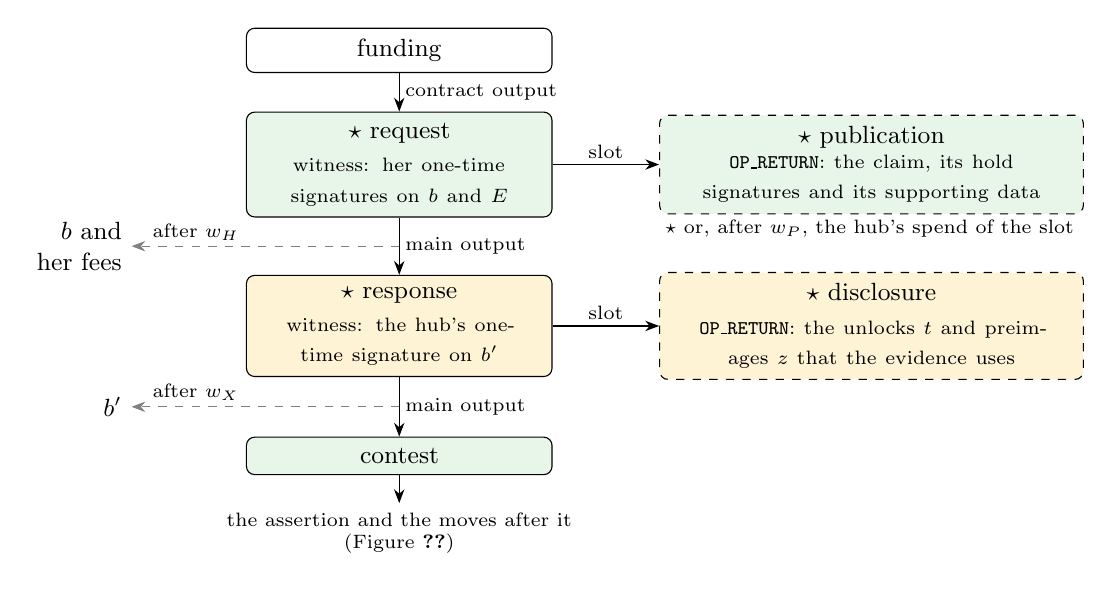
\begin{tikzpicture}[font=\small, >={Stealth[length=5pt]},
  box/.style={draw, rounded corners=3pt, inner sep=4pt, align=center, text width=36mm},
  hold/.style={box, fill=coop}, hub/.style={box, fill=hubc},
  free/.style={dashed, text width=51mm},
  lab/.style={font=\scriptsize, inner sep=2pt},
  pay/.style={align=right, font=\small}]
\node[box] (fund) at (0,0) {funding};
\node[hold] (req) at (0,-1.45) {$\star$ request\\[1pt]{\scriptsize witness: her one-time signatures on $b$ and $E$}};
\node[hub] (resp) at (0,-3.5) {$\star$ response\\[1pt]{\scriptsize witness: the hub's one-time signature on $\bresp$}};
\node[hold] (con) at (0,-5.15) {contest};
\node[hold, free, anchor=west] (pub) at (3.3,-1.45) {$\star$ publication\\[1pt]{\scriptsize \texttt{OP\_RETURN}: the claim, its hold\\signatures and its supporting data}};
\node[hub, free, anchor=west] (dis) at (3.3,-3.5) {$\star$ disclosure\\[1pt]{\scriptsize \texttt{OP\_RETURN}: the unlocks $t$ and preimages $z$ that the evidence uses}};
\node[font=\scriptsize, anchor=north west, inner sep=2pt] at (pub.south west) {$\star$ or, after $\wP$, the hub's spend of the slot};
\draw[->] (fund) -- node[lab, right] {contract output} (req);
\draw[->] (req) -- coordinate[pos=0.5] (m1) node[lab, right] {main output} (resp);
\draw[->] (resp) -- coordinate[pos=0.5] (m2) node[lab, right] {main output} (con);
\draw[->] (req) -- node[lab, above] {slot} (pub);
\draw[->] (resp) -- node[lab, above] {slot} (dis);
\draw[->, black!50, dashed] (m1) -- node[lab, above, text=black, pos=0.76] {after $\wH$} ++(-3.4,0) node[pay, left, text=black] {$b$ and\\her fees};
\draw[->, black!50, dashed] (m2) -- node[lab, above, text=black, pos=0.76] {after $\wX$} ++(-3.4,0) node[pay, left, text=black] {$\bresp$};
\draw[->] (con) -- ++(0,-0.6) node[below, align=center, font=\scriptsize] {the assertion and the moves after it\\(Figure~\ref{fig:dispute})};
\end{tikzpicture}
\caption{The transactions of a recovery up to the contest. An arrow is the spend of an output, and a dashed arrow a timeout, as in Figure~\ref{fig:dispute}. The holder's transactions are green and the hub's yellow, and the statement reads those with a star. The two with a dashed border are not in the contract's graph: one party alone signs each, when it publishes it. Fee outputs are left out.}
\label{fig:graph}
\end{figure}

What the request and the publication say does not depend on the chain. The program verifies her one-time signatures itself, and it accepts as her claim only data that hashes to the $E$ that she signed. For these two the chain settles whether she published and in which block: without her publication, the hub's own spend of the slot would stand in its place. The claim is judged on the chain up to that block, where the program also reads the heights that its locks refer to and the activations that it cites (Section~\ref{sec:interop}).

What the response and the disclosure say depends on the chain alone. Script verifies the hub's signature on $\bresp$ in the response, and each output of a payout of $\bresp$ opens to a signature under the same one-time key. The program does not verify the signature, since the hub runs the program and can sign any amount. The amount proved is the amount paid because the program reads $\bresp$ where the holder does, in the response on Bitcoin: with that signature she takes her outputs at once, and a second amount signed by the hub could move them only after the delay (Section~\ref{sec:rec}). A secret is public because it is in the spend of the response's slot. A proof for another amount, or with secrets that were not published, needs blocks that Bitcoin does not hold, with the contract's work on top, which our assumption excludes (Section~\ref{sec:model}).

Lichen's design for an amount chosen after the setup~\cite{delving} binds it otherwise: the party that did not choose the amount countersigns it with a one-time key, Script checks that the two signed values are equal, and the proof verifies the countersignature. Here the holder would sign $\bresp$ when she contests. This would free $\bresp$ from the assumption on private work, at the cost of a second signature and a comparison in Script, but not the publication or the disclosure, which the program reads from Bitcoin in either design.

\end{document}
